\documentclass[a4paper,12pt]{article}
%
%$Id: draft.tex,v 1.3 2004/03/08 15:19:37 rassy Exp $
%

\usepackage{ngerman}
\usepackage{graphicx}

\parindent0em
\parskip0.75\baselineskip

\newcommand{\code}[1]{\texttt{#1}}
\newcommand{\AEU}{AEU}

\title{Autoren-Entwicklungsumgebung (AEU) \\ -- Skizze --}
\author{Tilman Rassy, Ruedi Reiler, Helmut Vieritz}
\date{M"arz 2004}



\begin{document}

\maketitle

\section{Grundidee}
Die Autoren-IDE soll es offline erm"oglichen, die Inhalte des JAPS zu bearbeiten. Auf
Anforderung soll sie ihre Dokumente mit dem JAPS "uber das Internet abgleichen k"onnen.

\section{Funktionalit"aten}

\subsection{Navigation}

Die Navigation soll grafisch im Browser erfolgen. Sie soll Sections und Dokumente aller
Typen abdecken.

Im Fall der \emph{Linearen-Algebra-Sections} soll die Navigationsoberfl"ache an den
sog.\ "`W"urfel"' angelehnt sein, d.h.\ man soll sich "`im W"urfel bewegen"' k"onnen.
Nichtben"otigte Teile der Hierarchie sollen hierbei ausblendbar sein.

Steigt man bei der Section-Navigation bis zur untersten Ebene ab, sollen schliesslich die
Elemente angezeigt werden (mit Namen und Kategorie). Auf ein noch festzulegendes Maus-Event
(Mouseover?) soll dann eine Liste der zu dem Element geh"orenden Subelemente erscheinen (mit
Namen und Kategorie; Popup-Fenster). 

F"ur beliebige Dokumenttypen soll es zudem eine Listenansicht geben. Hierbei werden alle
Dokumente eines Typs aufgelistet. Bei Bildern und Applets sollen hierbei (auf Wunsch)
Thumbnails verwendet werden. Da die Dokumente, au\3er im Fall der Elemente, nicht
gegliedert sind, muss es eine Suchfunktion geben, damit der Autor die f"ur ihn relevanten
Dokumente ausw"ahlen kann.

F"ur ein Dokument sollen, nachdem es in der Navigation gefunden wurde, auf noch
festzulegende Maus-Events hin verschiedene Aktionen gestartet werden k"onnen. Dazu z"ahlen:
\begin{itemize}
\item Anzeige einer \emph{Info-Seite} des Dokuments. Zeigt alle Meta-Informationen an
  (gerenderte XML-Darstellung im Use-Mode \code{info}).
\item \emph{Ansicht} des Dokuments (Preview).
\item \emph{Bearbeiten} des Dokuments. Bei Elementen und Subelementen: "Offnen der
  TeX-Quelle in einem Editor.
\item Ggf.\ Anzeige einer \emph{Manual-Seite} zu dem Dokument. Diese enth"alt z.B.\ bei
  Applets Angaben, die der Autor zum Einbinden in sein Dokument ben"otigt, etwa Angaben
  "uber Parameter.
\item \emph{Einchecken} eines Dokument in den JAPS.
\end{itemize}

Bei Sections der untersten Ebene soll es ausserdem m"oglich sein, neue Elemente
anzulegen, allerdings nur f"ur privilegierte Benutzer.


\subsection{Redaktionelles System}

Das redaktionelle System soll alle organisatorischen Aspekte der Inhaltsentwicklung
betreuen. Dazu z"ahlen insbesondere:

\begin{itemize}
\item \emph{Versionsmanagement} -- Der Benutzer soll sich Versionsinformationen zu allen
  (lokalen) Dokumenten anzeigen lassen k"onnen. Vorbild: CVS, evtl.\ plus zus"atzliche
  Features (wer arbeitet sonst noch an dem Dokument? u."a.)
\item \emph{Bugreportsystem.} -- Aufgefundene Fehler in einem Dokument sollen registriert und an
  den Autor gemeldet werden k"onnen.
\item \emph{Redaktionelle Kontrolle} -- Dokumente m"ussen begutachtet und in ihren
  verschiedenen Stadien (s.u.) freigegeben werden, bevor sie schlie"slich "`offiziell"' im
  JAPS zur Verf"ugung stehen (Referee-System).
\end{itemize}

Die Oberfl"ache des Redaktionstools soll Tabellenform haben. Jede Zeile entspricht einem
Element oder Subelement. Letztere werden bei ihren Elementen angezeigt. Es soll folgende
Spalten geben:
\begin{enumerate}
\item \emph{name} -- Name des Elements bzw. Subelements.
\item \emph{category} -- Kategorie  (definition, theorem, motivation, \ldots)
\item \emph{components} -- Komponenten mit Typ, als Liste
\item \emph{comment} -- ein Text mit Kommentaren der Autoren und Gutachter, kann w"ahrend
  des Erstellungs- und Begutachtungsprozesses zur Kommunikation verwendet werden.
\item \emph{status} -- Status, m"ogliche Werte: open, draft, draft\_okay, implemented, bug,
  tested.\footnote{Die Bezeichnungen sind teilweise noch ungl"ucklich und bessere
    Vorschl"age sind willkommen}
\item \emph{draft\_by} -- Benutzer, der dieses Dokument entworfen hat.
\item \emph{draft\_okay\_by} -- Gutachter, der den Entwurf freigegeben hat.
\item \emph{implemented\_by} -- Autor(en) des Dokuments
\item \emph{tested\_by} -- Tester des Dokuments
\end{enumerate}


\subsection{Dokumentenbearbeitung}
Hierzu z"ahlen alle Funktionalit"aten, die zum Erstellen und Bearbeiten der Dokumente n"otig
sind. Insbesondere:

\begin{itemize}
\item \emph{Editieren von Dokumenten} - "Offnen von Dokumenten aus der Navigationsansicht
  heraus. Insbesondere soll es m"oglich sein, direkt aus dem Browser heraus einen Editor mit
  dem Dokument (bzw.\ seiner Quelle) zu starten.
\item \emph{Erzeugen neuer Dokumente} - "`Create New"' Button (o."a.) in der
  Navigationsansicht. Erzeugt leeres Dokument mit verf"ugbaren
  Metainformationen.
\item \emph{Einchecken von Dokumenten}
\item \emph{Preview von Dokumenten}
\item \emph{Konvertierung von MmTeX-Quellen}
\end{itemize}

%\subsection{Weiteres}
%Ist die IDE immer nur f"ur einen Autoren gedacht oder k"onnen mehrere gleichzeitig mit einer
%Umgebung arbeiten (Userverwaltung???)?

\section{Implementierung}

\subsection{Grundidee}

Auf dem Rechner des Autors wird eine spezielle Version des JAPS inklusive Datenbank
installiert, im folgenden \emph{Client-JAPS} genannt. Dazu kommen Frontend-Programme, in
erster Linie ein Browser und ein Editor.

Die bisherige, normale JAPS-Version wird im folgenden \emph{Server-JAPS} genannt.


\subsection{Beschreibung}

Die Datenbank entspricht der des Server-JAPS, jedoch wird auf die
Versionsverwaltung verzichtet. Sie enth"alt die lokalen Versionen der ausgecheckten
Dokumente. Bei wiederholter Bearbeitung werden diese "uberschrieben.

Die Synchronisation mit dem Server-JAPS erfogt per Client-JAPS-Server-JAPS-Kommunikation
(s.\ Grafik). Die Frontend-Programme kommunizieren nur mit dem Client-JAPS (und evtl.\
untereinander).

Es ist keine st"andige Netzverbindung zum Server-JAPS erforderlich. Diese wird nur zur
Synchronisation gebraucht.

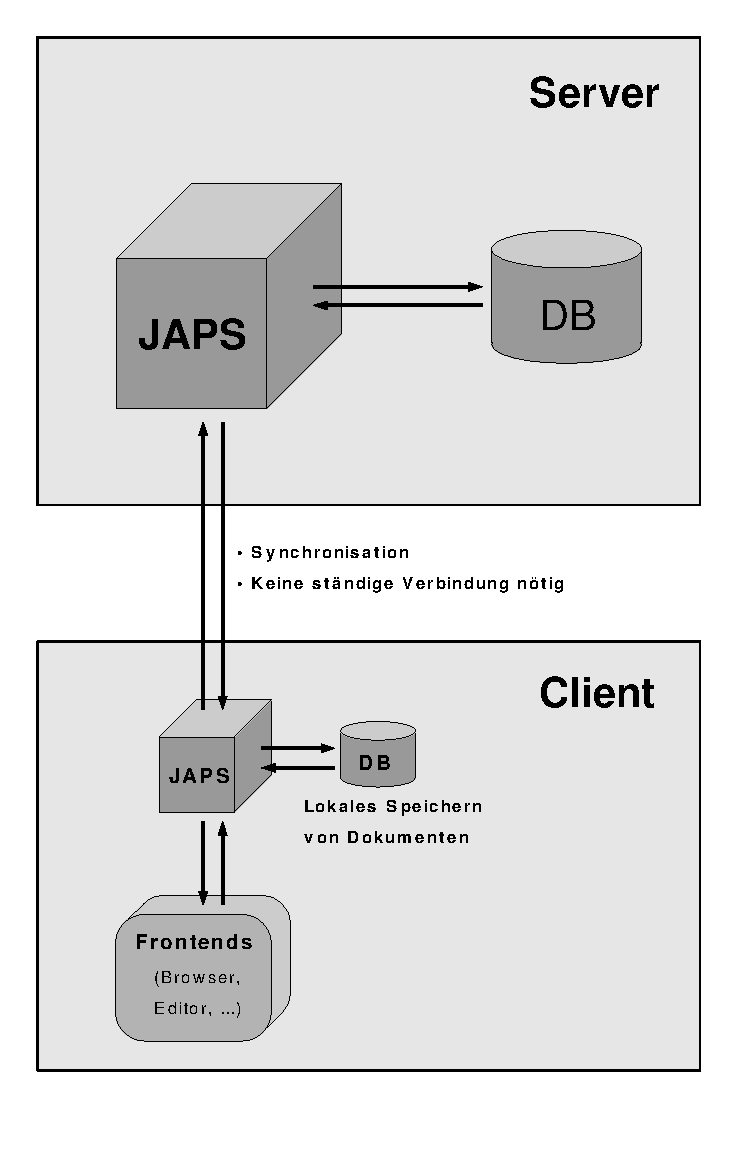
\includegraphics{authers_dev_env.pdf}


\end{document}
